\chapter{Transparent Decisions in Social Actors: Preferences}

Computational agents based on the BDI framework typically rely on abstract plans and plan refinement to reach a degree of autonomy in dynamic environments: agents are provided with the 
ability to select \textit{how-to} achieve their goals by choosing from a set of options. In this work we focus on a related, yet under-studied feature: \textit{abstract goals}. These constructs refer to the ability of agents to adopt goals that are not fully grounded at the moment of invocation, refining them only when and where needed: the ability to select \textit{what-to} (concretely) achieve at run-time. We present a preference-based approach to goal refinement,  defining preferences based on extended \textit{Ceteris Paribus} Networks (CP-Nets) for an AgentSpeak(L)-like agent programming language, and mapping the established CP-Nets logic and algorithms to guide the goal refinement step. As a technical contribution, we present an implementation of this method that solely uses a Prolog-like inference engine of the agent's belief-base to reason about preferences, thus minimally affecting the decision-making mechanisms hard-coded in the agent framework.


\section{Introduction}
% \Mos{It's not CP-Nets any more, mostly it's CP-Theories, need to change some text}

%new_commnent As computational agents intervene more and more in human activities, there is an increasing demand for human-oriented forms of programming, i.e. relying on concepts and abstractions mapping intuitively to what humans utilize to explain and direct their behaviour. The \textit{belief-desire-intention} (BDI) model of agency \cite{Rao1995}, centred around a general theory of mind \cite{bratman1987intention}, offers one of those views, and has been studied by the community since the 90s, resulting in the proposal and development of several platforms for agent-based programming (e.g. AgentSpeak(L)/Jason \cite{RaoAS1996,Bordini2005}, 3APL/2APL \cite{Dastani2APL}, GOAL \cite{Hindriks2009a}, IMPACT \cite{IMPACT}, JACK \cite{JACK}, Astra \cite{ASTRA}, LightJason \cite{Aschermann2018}, ASC2 \cite{mohajeriparizi_2020_run}---a  systematic review of logic-based MAS frameworks can be found in \cite{MASReview2021}).

Computational agents based on the BDI framework typically rely on abstract plans and plan refinement to reach a degree of autonomy in dynamic environments. In practice, relative autonomy in this context consists in the ability of an agent to select \textit{how-to} achieve their goals by choosing from a set of options. BDI agent scripts typically consist of hierarchical, partial, abstract plans. This contrasts with classic forms of planning, providing agents with fully-grounded policy, designed to reach a certain specific objective. 

This work focuses on a related, yet under-studied feature: % present in BDI frameworks, particularly in those based on the AgentSpeak(L) language:
%(although already present in frameworks as those based on the AgentSpeak(L) language)
\textit{abstract goals}. These constructs refer to the ability of agents to adopt goals that are not fully grounded at the moment of invocation, refining them only when and where needed, that is, the ability to select \textit{what-to} (concretely) achieve at run-time. Examples of abstract goals can be found typically in \textit{activity}-level characterizations of behaviour, e.g. walking (where?), eating something (what?), meeting someone (who?), selling (what? to whom?), etc. 

The specification of abstract goals is a feature already present in some agent frameworks as those based on the AgentSpeak(L) language, albeit they rely on simplistic mechanisms for goal refinement. The present work aims to cover the goal refinement step (from abstract goals to concrete goals) as part of the agent's decision-making cycle. For doing so, 
we present a preference-based approach to goal refinement. We start from defining preferences based on \textit{Ceteris Paribus} Networks (CP-Nets) \cite{Boutilier2004}---more precisely, in the extended form of \textit{Ceteris Paribus} Theories (CP-Theories) \cite{Wilson2004}---and we consider the established CP-Net logic and algorithms to guide the goal refinement of the agent. At implementation level, our target is an AgentSpeak(L)-like \cite{RaoAS1996} agent programming language. Since Jason \cite{Bordini2005},  AgentSpeak(L) programs are enriched with Prolog rules and facts for knowledge-level processing, occurring e.g. for testing context conditions during the plan selection phase. We present therefore an implementation of a preference-based goal refinement method that solely uses a Prolog-like inference engine of the agent's belief-base to reason about preferences, requiring only a minimal modification to the decision-making mechanisms hard-coded in the agent framework. To achieve this, a transformation method is proposed to map an extended version of CP-Nets and CP-Theories into Prolog facts and rules for the script of the AgentSpeak(L) agent, as well as a Prolog implementation of the algorithms necessary to reason with preferences.

The chapter proceeds as follows: section \ref{sec:2} provides a background about the concepts used in this work; section \ref{sec:method} presents the method and examples for preference-based abstract goal refinement in AgentSpeak(L) agents; section \ref{sec:implementation} describes a practical implementation of this method, and section \ref{sec:discuss} elaborates a discussion and conclusion over the proposed method. 

% \begin{comment}

% [Copied]

% In the last decades several attempts have been made to move from machine-oriented views of programming towards concepts and abstractions that more closely reflect the way in which humans conceive the world. In particular, the \textit{belief-desire-intention} framework (BDI) \cite{Rao1995}, building upon a theory of mind \cite{bratman1987intention}, has been introduced to provide a basis for the implementation of computational agents that exhibit rational behaviour, using the same representations that we typically use to address human behaviour. % Additionally, from a modeling  standpoint, the BDI framework offers a cognitive model for agent-based modelling (ABM) \cite{balke2014}, 
% %\subsubsection{Why prioritize BDI scripts with preferences}
% In the %related 
% decision-making literature, instead, particular attention is given to the role of preferences: any model of agency involving decision-making is deemed to abide the agent's preferences \cite{Pigozzi2016}. This does not imply that any model of agency will rely on explicit preferences, rather it affirms the general principle that when there are multiple goals that should be achieved (or multiple ways to achieve a certain goal or even multiple sets of states that can be reached) the best course of action is the one that abides the most to the agent's preferences \cite{Pigozzi2016}.
% In practice, preferences can vary from the implicit ``maximize utility" of optimizing agents \cite{Nunes2014} to explicit preferences specified in a preference representation language \cite{Dasgupta2010,Visser2011}. 
% % BDI agent execution architectures, more often than not, rely on logical constructs for modeling the agents' mental components, see e.g. the critical overview given in \cite{Herzig2018}. 
% %Unexpectedly, none of the main BDI languages presented in the literature support explicit preferences. %Decisions between alternative choices (in our case, for plan selection) are generally based on implicit forms of preferences like sequential ordering (e.g. of plan specifications).% Only a few works have investigated a potential role for explicit preferences in BDI agents \cite{Dasgupta2010,Visser2011,Nunes2014,Mohajeri2019}

% \end{comment} 

%%%%%%%%%%%%%%%%%%%%%%%%%%%%%%%%%%%%%%%%%%%%%%%%%%%%%%%%%%%%%%%%%%%%%%%%

\section{Background} 
\label{sec:2}
%\Mos{we need to make a choice (later) to keep the related works here or move them to discussion. Some like GAI networks or other preference frameworks do not make much sense in discussion, but other BDI/Pref ones do for comparison} 
% This section provides an overview of the concepts and methods on which our contribution builds upon. Most of these sections are succinct version of what presented in \cite{Mohajeri2019}.
% \vspace{0pt} \noindent \textbf{BDI Agents} \quad
\subsection{Abstract Plans in BDI Agents}

Agents specified following the BDI paradigm are characterized by three mental attitudes. Beliefs are facts that the agent believes to be true. Desires capture the motivational dimension of the agent, typically conflated with the more concrete form of \textit{goals}, representing procedures/states that the agent wants to perform/achieve. Intentions are selected conducts (or \textit{plans}) that the agent commits to (in order to advance its desires). 

Since their origin \cite{Rao1995}, the essential feature associated to BDI architectures is the ability to instantiate abstract plans that can (a) react to specific situations, and (b) be invoked based on their purpose. Consequently, the BDI execution model often relies on a \textit{reactive} model of computation, usually in the form of some type of \textit{event-condition-action} (ECA) rules often referred to as \textit{plans}. Plans are uninstantiated specifications of the \textit{means} (in terms of course of actions) for achieving a certain \textit{goal} \cite{Rao1995}. These constructs represent the procedural knowledge (\textit{how-to}) of the agent. There are multiple proposals in the literature for programming language and architecture of BDI agents, the most commonly used being AgentSpeak(L) \cite{RaoAS1996}, which will serve as basis for the present proposal. % is also based upon the AgentSpeak(L) language and a more detailed description of it is presented in section \ref{ssec:agentspeak}.

%\vspace{5pt} \noindent \textbf{Preferences in BDI agents} \quad
% Multiple BDI languages and frameworks have been introduced in the literature, typically in form of \textit{Multi-Agent System (MAS)} frameworks, such as AgentSpeak(L)/Jason \cite{RaoAS1996,Bordini2005}, 3APL/2APL \cite{Dastani2APL}, GOAL \cite{Hindriks2009a}, IMPACT \cite{IMPACT}, JACK \cite{JACK}, Astra \cite{ASTRA}, LightJason \cite{Aschermann2018}, and ASC2 \cite{mohajeriparizi_2020_run}. 

%All of these frameworks  In current BDI implementations, preferences between these optional conducts are specified through a static ordering assigned by the programmer, typically via the ordering of rules in the code: the higher a rule is in the script, the more priority the associated plan has. 

%This explains why most current frameworks including Jason \cite{Bordini2005}, 2APL \cite{Dastani2007}, ASC2 \cite{mohajeriparizi_2020_run}, etc. are genuinely \textit{reactive}: the scripts are interpreted without the need for any additional introspection/deliberation steps. However, these frameworks also expose \textit{plan selection} functions that can be modified to implement alternative mechanism for goal-plan rule selection during the deliberation cycle which can be considered as a type of meta-programming over agent scripts. % As it was said before, this approach has the positive features of simplicity, readability and performance while having the issue that these order-based preferences stay in the mind of programmer, and are not represented as explicit preferential knowledge.
% For more clarity, to better separate goal-adoption from the treatment of primitive actions, we will not consider primitive actions as part of preferences. 
%[???] 
%The latter option has been taken by almost all works adding explicit preferences to BDI agents \cite{Visser2011,Dasgupta2010,Nunes2014}: the selection of the most preferred alternative is taken as a \textit{reflective} process, where preferences provide a \textit{rationale} to be applied online during the agent's deliberation cycle.  The idea of relying on an offline step is instead proposed also in \cite{Mohajeri2019}, but they only focused on \textit{procedural preferences} (``I prefer to be doing $a_i$ rather than doing $a_j$"), which have a different level of abstraction w.r.t. to declarative preferences (``I prefer being in state $s_i$ rather than being in state $s_j$"). % This chapter focused instead on \textit{declarative preferences}, i.e. about states of the world (``I prefer being in state $s_i$ rather than being in state $s_j$"). For this purpose, we used the notions of (1) \textit{declarative goals} (``want-to-be'' goals), and of (2) \textit{post-condition} or effect specification of \textit{primitive actions}. 
%Modifying the deliberation cycle by adding run-time reflective steps (as a complex preference checking and related plan selection algorithms) is generally detrimental to reactivity

%$\paragraph{Reasoning cycle}

%There is an extensive literature between BDI agent programs and HTNs (\textit{hierarchical task networks}) planning domains \cite{DeSilva2019,Meneguzzi2013}.
%Solutions to classic planning problems are concrete sequence of actions, to be performed by the agent to reach a certain goal. 
%Plan refinement \cite{Kambhampati1997} considers the set of all action sequences and manipulates it progressively following diverse strategies, narrowing it down to the set of possible solutions. The manipulation occurs via partial plans, which for this reason can be seen as behavioural constraints. % Yet, planning approaches typically do not consider abstraction of actions  \cite{Hoffmann2006}, nor of goals.
%Rather than looking at all solutions, and then evaluating those to select the best one, the decision-making cycle of reactive BDI agents---as those specified in AgentSpeak(L)---selects the first available plan. From this point of view, they can be seen as ``reactive planning systems'' \cite{Wooldridge1995a}. However, differently from planning systems, BDI agents do not form a complete solution up-front, but unveil it on the fly, so it may happen that, given a problem, a solution is partially formed, partially executed, when an external event changes the search towards another problem.


%\Gio{[Here there should be more detail about the decision-making cycle used in AgentScript, so that people understand why the Prolog mechanism is fine as a solution.]}
%\Mos{moved to 3.1, so we can focus on AgentSpeak}

%\vspace{5pt} \noindent \textbf{Preference languages} \quad

\subsection{Preference Languages}
Preferences play a crucial role in decision-making \cite{Pigozzi2016}. Several models of preferences have been presented in the literature (e.g. on decision-making, planning, etc.), with various levels of granularity and expressiveness (see e.g. \cite{Domshlak2011}). The most straightforward \textit{quantitative} approaches are based upon \textit{utility theory} and related forms of decision theory. % A hybrid quantitative method is provided by PDDL3 \cite{Gerevini2005}, an extension of the \textit{planning domain definition language} (PDDL) \cite{McDermott1998}. Although based on qualitative descriptions, these preferences are considered quantitative \cite{Baier2007} because the valuation of each preference is expressed with a numerical value. 
% In \cite{Cranefield2017} one can find some examples of integration of these types of preferences in a BDI architecture.
Although utility-based approaches bring clear computational advantages, they also suffer from the non-trivial issue of translating users' preferences into utility functions. 

%This explains the existence of a family of \textit{qualitative} or hybrid solutions. A hybrid method is provided by PDDL3 \cite{Gerevini2005}, an extension of the \textit{planning domain definition language} (PDDL) \cite{McDermott1998}.% Although based on qualitative descriptions, these preferences are considered quantitative \cite{Baier2007} because the valuation of each preference is expressed with a numerical value.
%, as LPP \cite{Bienvenu2006} and PDDL3 \cite{Gerevini2005}. 

This explains the existence of a family of \textit{qualitative} or hybrid solutions. % that allow for explicit specification of preferences. 
The \textit{logical preference description} (LPD) language \cite{Brewka2004} uses ranked knowledge bases alongside preference strategies to present preference descriptions. The LPP language \cite{Bienvenu2006} is a first-order preference language defined in situation calculus to reason about conditional and qualitative preference.
%Proposals exist for integrating LPP in BDI agents \cite{Visser2011}. 
Other preference models, such as GAI networks \cite{Gonzales2004}, CP-Nets \cite{Boutilier2004} and qualitative preference systems (QPS) \cite{Visser2012QPS}, have been specifically introduced for taking into account dependencies and conditions between preferences. GAI networks build upon the assumption of \textit{generalized additive independence}, and in doing so they enable computing the utility contribution of every single attribute/subset of attributes. QPS offers a framework for representing multi-criteria preferences based on a lexicographic rule which combines basic preferences over variables, and a cardinality-based rule which counts criteria that are satisfied; QPS have been extended with goal-based preferences \cite{Visser2013QPS}, allowing to define preferences from the context of goals.

% Whereas CP-nets have weak constraints,  (they can be seen as the preferential counterpart of Bayesian networks). CP-nets and GAI-networks share possibility to be illustrated as intuitive graphical models. 
In the present work, we decided to focus on CP-Nets, and their extension CP-Theories \cite{Wilson2004}, for two main reasons: they rely on weaker assumptions, and exhibit primarily a qualitative nature. 

%To our knowledge, \cite{Mohajeri2019} was the first attempt to introduce this type of representational models in a BDI architecture, although focusing only on procedural preferences.
%This work continues the previous effort by considering declarative preferences.

\subsubsection*{Ceteris Paribus networks (CP-Nets) }
Conditional \textit{ceteris paribus}  preferences networks (CP-Nets) are a compact representation of preferences in domains with finite \textit{attributes of interest} \cite{Boutilier2004}. An attribute of interest is an attribute in the world (e.g. \textit{restaurant}) that the agent has some sort of preference over its possible values (e.g. \textit{italian} and \textit{french}). CP-Nets build upon the idea that most of the preferences people make explicit are expressed jointly with an implicit \textit{ceteris paribus} (``all things being equal'') assumption. For instance, when someone says ``I prefer a French restaurant over an Italian one'', they do not mean at all costs and situations, but that they prefer a French restaurant (over an Italian one), all other things being equal. An example of \textit{conditional preference} is ``If I'm at a French restaurant, I prefer fish over meat''.
CP-Theories \cite{Wilson2004} extend CP-Nets adding stronger conditional statements with the construct ``\textit{regardless of}'', allowing some attributes to be released from the equality rule. 

In general, CP-Nets can be associated with two tasks: (1) finding the most preferred outcome on a certain domain of variables (2) comparing two outcomes with different criteria. Both CP-Nets and CP-Theories provide efficient algorithms for these tasks.

%\Gio{[I would introduce here more about the formalism]}
%\Gio{[Which are the typical inferences to be performed on CP-nets? Which are the tools? complexity?]}

\subsubsection{Preferences in BDI Agents}
Goals are used to identify desired states or outcomes, and preferences are used to identify more (or less) desired states or outcomes. While goals are a central aspect in BDI agents, so far, none of the main BDI frameworks and languages include preferences as part of the definition of the agents. This explains why there exist already previous studies that, like this work, attempt to  enhance BDI agents with explicit preferences. Visser et al. \cite{Visser2011,Visser2016} present an approach to embed preferences defined in the LPP language into BDI agents to guide plan selection. Nodes in the goal-plan tree of the agent are annotated by the designer about the effects of that plan and then this information is propagated automatically to other nodes in the tree at compile time. Then, at run-time, the agent uses the LPP logic to select the most preferred plan for a goal based on this information. 
Dasgupta et al. \cite{Dasgupta2010} proposes a lookahead method to enhance AgentSpeak(L) agents with constraints and objectives that the agent can use for plan selection at run-time; their approach also requires annotations for plans to reason about the preferability of plans. Mohajeri et al. \cite{Mohajeri2019,Mohajeri2020} add preferences in form of CP-Nets in AgentSpeak(L)-like agents, however, their approach consider a cross-compilation step: %that creates a conditional ordering over the plans of the agent. %with respect to a set of preferences. 
they annotate primitive actions of agents with their expected effects, and this information is then propagated through the goal plan tree to create a conditional ordering between plans. Padgham et al. \cite{Padgham2013} add situational preferences as part of plan definitions in a BDI language. The agent can use them to quantify the value of each plan at run-time. Their method is similar to this work in the sense that it does not require any lookahead, but it is different because they add preference valuations as part of each plan, which are then used in plan selection with the implicit preference of maximizing them---this makes the approach essentially a quantitative one.

%\subsection{Autonomy
%\Gio{[Perhaps something should be here about what we mean as autonomy {or perhaps this is good for the conclusion}.]}
%\Mos{Giovanni can write this}

% As this work is an initial step in integrating preferences in BDI scripts the full power of CP-nets and its extensions is not utilized yet. % the point here is to show as a proof of concept how such compact presentation can be used in this manner.
%An attribute $A$ is said to be the parent of attribute $B$ if preferences over $B$ are conditional over values of $A$. 


\section{Method}
 \label{sec:method}
% \color{lightgray}
% Highlight Points:
% \begin{itemize}
%     \item Explicit Preferences
%     \item CP-nets
%     \item preferability vs. applicability
%     \item Comparing our CP-net with original
%     \item Preferences are written in Logic form
%     \item Reasoning only happens inside agent's belief base / minimal extra machinery
% \end{itemize}

\subsection{AgentSpeak(L) Agents}
\label{ssec:agentspeak}
While this work mainly focuses on ASC2 as the BDI framework, the methods proposed in this chapter target any frameworks that utilize AgentSpeak(L). The main point of interest in BDI reasoning cycle for the preference reasoning approach proposed in this chapter is the plan instantiation process. This process, as it was briefly introduced in the previous section, starts when an event is selected for processing. Firstly the event is unified with the triggering events of the plans in the plan library. The ones that do unify are called relevant plans and the resulting unifier is called the relevant unifiers. Then, for each relevant plan, the relevant unifier is applied to its context condition and the result is queried against the belief base to create zero or more substitutions such that the context is a logical consequence of agent's current belief. The composition of relevant unifier with each substitution is called an \textit{applicable unifier}.  The following definitions apply:


% Based on the definitions proposed by Rao et al. in \cite{Rao1995,RaoAS1996}, an agent consists of a set of beliefs $B$ called belief base, a set of plans $P$ called plan library, a set of events $E$, a set of actions $A$, a set of intentions $I$, and three selection functions: $S_E$, that selects events for processing; $S_O$ selects one of applicable plans for instantiation, and, $S_I$ that select an intention. 

\begin{definition}
[Plan] A (reactive) plan is specified by $e : C \Rightarrow H$ where $e$ is a triggering event, $C$ is a formula capturing context conditions, and $H$ is a sequence of sub-goals or actions to be performed at the occurrence of the trigger event.
\end{definition}

\begin{definition}
[Relevant plan] A plan in the form of $e : C \Rightarrow H$ is a \emph{relevant plan} with respect to an event $\epsilon$ iff there exists a most general unifier $\sigma$ such that $\epsilon\sigma = e\sigma$. Then, $\sigma$ is referred to as the \emph{relevant unifier} for $\epsilon$.
\end{definition}

\begin{definition}
[Applicable plan] A plan in the form of $e : C \Rightarrow H$ is an \emph{applicable plan} with respect to an event $\epsilon$ iff there exists a relevant unifier $\sigma$ for $\epsilon$ and there exists a substitution $\delta$ such that $C\sigma\delta$
is a logical consequence of belief base $B$. The composition $\sigma\delta$ is referred to as the \emph{applicable unifier} for $\epsilon$ and $\delta$ is referred to as a \emph{correct answer substitution}.
\end{definition}


%As for each event there could be multiple applicable unifiers, the selection function $S_O$ chooses one of these plans or options and applying the applicable unifier to that plan creates an instantiated plan, i.e, an intended means or the event which will be added to a new or existing intention. Then the $S_I$ function selects an intention which will be executed. We will now consider an example agent to illustrate the plan instantiation process.


% As this work focuses on the goal refinement, the following formal definitions namely plans, relevant plans, and applicable plans are reiterated from \cite{RaoAS1996}. 





% \Gio{[here we should write a bit about variables, constants, unification and unifiers.]}
% \Mos{Giovanni can write this}


%\noindent For the given definitions, only relevant plans may be applicable. 

\subsubsection*{Example 1}
Imagine again the domestic robot from the previous chapter, an agent that upon request, can go to a restaurant and order a three-course meal. This time the agent's plans and beliefs are expanded to give it more choice. The script for such agent is presented in Listing \ref{lst:script_1}.
%\footnote{%In the excerpts we modified 
%ASC2 slightly modifies the AgentSpeak(L) syntax, replacing ``\texttt{<-}'' with ``\texttt{=>}'', to further distinguish the reactive, forward nature of these rules w.r.t. the backward chaining derivation of Prolog rules ``\texttt{:-}''.} 
The agent has two plans for going to a restaurant and ordering a meal: the first plan (P1) is \textit{applicable} if the agent is not at a restaurant at the moment, which means a step of moving (\asc{#move_to} primitive action) is needed prior to ordering the meal; the second plan (P2) is applicable if the agent is already at the restaurant which means the agent will just adopt the goal of ordering the meal. There is also one plan for ordering the meal (P3) which is applicable if the agent has the belief that the meal it wants to order exists.
\begin{listing}[t]
\centering
\begin{minted}[fontsize=\small]{prolog}

% (P1) 
+!go_order(Loc,Meal) :
    restaurant(Loc) & not at(Loc) =>
        #move_to(Loc);
        !order(Meal).
% (P2) 
+!go_order(Loc,Meal) :
    restaurant(Loc) & at(Loc) => 
        !order(Meal). 
% (P3) 
+!order(meal(S,M,W)) : 
    meal(S,M,W) => 
        #ask_waiter(meal(S,M,W)).
\end{minted}
    \caption{Reactive Plans of Food-ordering Agent}
    \label{lst:script_1}
\end{listing}%
\noindent Suppose the agent selects an event with the trigger: 
\begin{minted}[fontsize=\small]{prolog}
!go_order(french,meal(veg,meat,white))
\end{minted}
For this event, both plans (P1) and (P2) are relevant with unifier $\sigma$:
\begin{minted}[fontsize=\small]{prolog}
{Loc/french, Meal/meal(veg,meat,white)}
\end{minted}
Assuming that the belief base of the agent contains the beliefs \asc{restaurant(french)} (meaning that there exists a French restaurant) and \asc{at(home)} (meaning that the agent is at home), then only the first plan will be an applicable plan for this event, and the applicable unifier will be the same as the relevant unifier. This entails that only plan (P1) will be instantiated as: 
\begin{minted}[fontsize=\small]{prolog}
+!go_order(french,meal(veg,meat,white)) :
    restaurant(french) & not at(french) =>
    #move_to(french);
    !order(meal(veg,meat,white)).
\end{minted}

Note that in case the agent had more than one applicable unifiers, meaning it had more than one option to react to this goal, then the $S_O$ function would have been called to select one of the options. 


\subsection{Abstract Events, Abstract Goals}
Partial autonomy in dynamic environments is considered a core attribute of BDI agents, and this is in fact one of the reasons that separates plan refinement in BDI agents from classical planning approaches \cite{DeSilva2004}. While the idea of choosing between distinct plans to achieve a certain goal---typically referred to as plan selection---has been investigated by the community as the principal point of autonomous choice in BDI agents, there is indeed another important type of autonomy embedded in BDI agents: abstract events. While the previous example only exhibited fully grounded events, BDI agents, in particular those derived from  AgentSpeak(L)  \cite{Rao1995,RaoAS1996} 
%and by extension  available in  \cite{}, 
can indeed handle abstract events, referring to situations where an event contains unbounded variables and these variables can be grounded by different means such as context conditions of plans or test goals at any level in the plan refinement of the event. It can be argued that if plan selection promotes autonomy in the \textit{how-to} dimension of the agent, abstract events, including the invocation of abstract goals, promote autonomy in selecting (concretely) \textit{what-to} with it.

\subsubsection*{Example 2}
Consider the same agent presented in listing \ref{lst:script_1}. This time we assume the agent has more information about the environment: it has beliefs about two types of soups, two types of main course, two types of wine, two restaurants, also it believes that it is standing already in one of the restaurants (the \texttt{french} one), and finally it has an inferential rule for which all possible triple of soup, main course and wine form  a meal combination. Those beliefs are presented as in listing~\ref{lst:beliefs_1}.

\begin{listing}[t]
\centering
\begin{minted}[fontsize=\small]{prolog}
main(fish). main(meat). soup(veg). soup(fish).
wine(white). wine(red).
restaurant(french). restaurant(italian).
at(french).
meal(S,M,W) :- soup(S), main(M), wine(W).
\end{minted}
    \caption{Beliefs of Food-ordering Agent}
    \label{lst:beliefs_1}
\end{listing}


Now assume the agent receives an abstract event \asc{!go_order(L,M)} which basically puts no constraints over where the agent should go and what it should order, and so gives it full autonomy to choose how to proceed. When the agent receives this event, both plans P1 and P2 are considered relevant plans with unifier \asc{{Loc/L, Meal/M}}. But considering the context conditions and the belief base, P1 will be applicable with unifier \asc{{Loc/italian, Meal/M}} and P2 with \asc{{Loc/french, Meal/M}} (note that in both cases the second parameter is not grounded as it is unified to another variable). At this point the agent's reasoning engine needs to use its plan selection function to choose one of the two plans. In both cases, the next event for the agent will be \asc{!order(M)} and P3 is a relevant plan for this event with unifier \asc{{M/meal(S,M,W)}}.  Taking into account the unification occurring at context conditions, this event will have in principle $2^3 = 8$ different applicable unifiers with all possible combinations for the meal, e.g: \asc{{M/meal(veg,fish,white)}}, for which, again, the plan selection function needs to choose an option to start the actual execution. The goal-plan tree of this abstract goal can be seen in Figure~\ref{fig:gp-tree}.

\begin{figure}[!t]
  \centering
  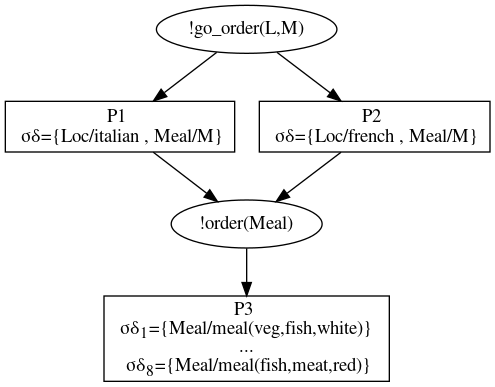
\includegraphics[width=0.70\linewidth]{ch3/outfile.png}
  \caption{Goal-Plan Refinement of the Agent}
  \label{fig:gp-tree}
\end{figure}

In current implementations of BDI frameworks based on AgentSpeak(L), the three selection functions $S_E$, $S_O$, $S_I$ (respectively for events, plans/options, and intentions) are typically exposed as abstract functions that the designer can override to implement any type selection function. Although this approach promotes flexibility, the fact that part of the decision-making remains external to the agent script reduces readability, encapsulation, and transparency of the agent programs, and makes the control more opaque to the designer. For these reasons, the selection functions hardcoded should be kept as simple as possible.

Default implementations are based on selecting the first available option, which is indeed a good example of simplicity.
If we apply the default implementation also on this example, the first applicable unifier for \asc{!go_order(L,M)} is \asc{{Loc/italian, Meal/M}}, and the first applicable unifier for \asc{!order(S,M,W)} is \asc{{M/meal(veg,fish,white)}}.  %\Mos{Maybe you want to change this)}

%\Gio{[Here we should write that current execution of abstract plans do not look for all 8 configurations, they just take the first one which is retrieved satisfying the context conditions (typically depending on the order of beliefs specified in the program).}

\subsection{CP-Nets and CP-Theories}
\label{ssec:prefs}
%Recalling on the CP-Theories \cite{Wilson2004}, assume a set of variables $X \in V$ each having a set finite set of values $x$, deonted $Dom(X)$, called the \textit{domain} of $X$. A value $u$ for $U \subseteq V$ associates with every $X \in U$ a value of $X$. The set of all values $u$ for $U$ is denoted $Dom(U)$, called the domain of $U$ and $\top$ the only value of $U=\emptyset$. A conditional preference $\lambda$ on $V$ is denoted by $u:x \succ x'[W]$, where $U \subseteq V$, $u \in Dom(U)$, $X \in V - U$, $x,x' \in Dom(X)$, and $W \subseteq V - (U \cup \{X\})$. This preference relation means given $t \in Dom(T)$ where $T=V-(U\cup\{X\}\cup W)$, then $x$ is preferred to $x'$, irrespective of the value of $W$. CP-Nets \cite{Boutilier2004} can be presented with $W=\emptyset$.

%Based on this definitions, an outcome $o \in Dom(V)$
%\Mos{CP-nets and CP-Theories got very much intertwined here, need to clear up}

In order to specify preferences, we start from the definition of CP-Nets given in \cite{Boutilier2004}. Given a set of variables $X \in V$, each having a finite set of values $x$, conditional preference statements are in the form $u : x \succ x'$, where $x$, $x'$ are assignments of a variable $X \in V$, and $u$ is an assignment to a set of variables $U \subseteq V$ (parents of $X$). The interpretation of this statement is that given $u$, then $x$ is preferred to $x'$ all else equal, meaning, for all assignment $s$ of the set of variables $S$, where $S = V - (U \cup \{X\})$, $sux$ is preferred to $sux'$, where $sux$ and $sux'$ are two \textit{outcomes} (complete assignment) to all variables of $V$. 
CP-Theories are introduced in \cite{Wilson2004} to extend CP-Nets with \textit{stronger conditional statements}. These include preferential statements in the form $u : x \succ x' [W]$, where $W \subseteq V$ which interprets that for all assignments $w,w'$ to variables of $W$ and assignments $t$ to variables of $T = V - (U \cup {X} \cup W)$, then the outcome $tuxw$ is preferred to the outcome $tux'w'$. This means that given $u$ and any $t$, then $x$ is preferred to $x'$ \textit{regardless} of assignments to $W$.



%It is shown that with both CP-Nets and CP-Theories, a set of such preference statements $\Lambda$ generates a partial ordering between all the outcomes of $V$, if $\Lambda$ is consistent, where consistency corresponds to the preference relations being acyclic with respect to the parent child relations of the variables. 
Assuming $\Lambda$ is a set of acyclic (with respect to parent-child relations) preference relations over variables of $V$, and considering $o,o'$ are outcomes of $V$, then we say $\Lambda \models o \succ o'$ iff $o \succ o'$ satisfies every preference statement in $\Lambda$. 
%$\Lambda$ is satisfiable iff there exists a preference ranking $\succ$ over the outcomes of $V$ that each $o \succ o'$ satisfies each of the preference statements of $\Lambda$. It is said that $\Lambda \models o \succ o'$ iff $o \succ o'$ holds in every preference ordering that satisfies $\Lambda$. 
Then $o$ and $o'$ can have one of the possible relations according to $\Lambda$: either $\Lambda \models o \succ o'$; or $\Lambda \models o' \succ o$; or $\Lambda \not\models o \succ o'$ and $\Lambda \not\models o \succ o'$. The third case means there is not enough information to prove either outcome is preferred. 

Based on these definitions, two distinct ways for comparing outcomes are proposed in \cite{Boutilier2004}:
\begin{itemize}
    \item Dominance queries: Asking if $\Lambda \models o \succ o'$ holds, which is referred to as $o$ is preferred to and \textit{dominates} $o'$.
    \item Ordering queries: Asking if $\Lambda \not\models o' \succ o$ holds, which is referred to as $o$ is preferred to $o'$.
\end{itemize}
Although ordering queries are weaker than dominance queries, they are still sufficient in many applications, and will be used in this work. In particular, if an outcome $o$ is present such for all other outcomes $o'$ we have $\Lambda \not\models o' \succ o$, then we say $o$ is \textit{undominated} or \textit{most preferred} with respect to $\Lambda$.
%One of the main usages of such partial ordering is comparing outcomes, The are two distinct ways proposed by \cite{Boutilier2004}

All through this work, and for the sake of simplicity, only strict preferences $\succ$ are considered. Nevertheless, these semantics are shown to be extendable to weak preferences $\succeq$ and indifference $\sim$ in both CP-Nets and CP-Theories.

%While the idea of integrating CP-Nets (and CP-Theories) with BDI programs have been suggested before \cite{Mohajeri2019,Mohajeri2020}, there are important distinctions between the logic and algorithms defined for CP-Nets and those of BDI agents or even more broadly logic programs that need to be addressed. Firstly, by definition, CP-Nets rely on a closed world assumption, which means they assume a single static set of variables $V$ (or \textit{features} or \textit{attributes}) as the decision domain and all of the variables appearing in a conditional preference statement (or rule) should be part of $V$. Secondly, they focus attention on single-stage decision problems with complete information, ignoring any issues that arise in multi-stage, sequential decision analysis and any considerations of risk that arise in the context of uncertainty \cite{Boutilier2004}.% which means preference rules create a hierarchy between these variables.


%Contrary to CP-Nets, a BDI agent deals with many related or independent sets of variables in their decisions and can not be limited to one set. Also, a dynamic agent's factual, inferential, procedural or even preferential knowledge about the environment can be subject to revisions in the its life-cycle and it can not be assumed that all the variables are fully known at any point. Furthermore, BDI agents are designed to act in dynamic environments with incomplete information and uncertainty, and more often than not, a BDI agent deals with these issues via multi-stage decision making and dynamic reactions to the environment such as incremental plan and goal refinement and even failure handling.
\subsubsection{Embedding in BDI agents}
\label{sssec:transform}
To transform CP-Theories to a formalism that can be used with the Prolog-like inferential systems as those used in AgentSpeak(L) agents, one should look at what needs to be decided in the process of goal refinement. An agent may have dynamically interconnected beliefs about the environment, but when it is deciding on what is the most preferred approach to partially ground the variables of an event or goal in the form of e.g $!g(v_1,...,v_n)$, only the parameters of that goal are relevant to %part of 
the decision. Theoretically, in this approach we do not have only one CP-Theory, but each distinct goal/event has zero or more inferred CP-Theories from the set of all preference statements. 

In this work, the preferences of an agent are presented in a different notation from that of CP-Nets and CP-Theories, but more similar to OCP-Theories in \cite{DiNoia2015}.

A conditional preference statement $\lambda$ of the agent can be expressed in the form of inferential rules such as:
\begin{equation*}
    G \succ G' \leftarrow C
\end{equation*}
where $G,G'$ are either belief predicates in the form $g(v_1,...,v_n)$ and $g({v}_1',...,{v}'_n)$, or triggering events in the form $!g(v_1,...,v_n)$ and $!g({v}'_1,...,{v}'_n)$ (or any other type of trigger, $?,+,-$). Each $v_i$ and ${v}_i'$ can be either a (partially) ground term, a named variable or an anonymous variable (underscore, ``\texttt{\_}''), and $C$ is an arbitrary logical expression that \textit{activates} the preference statement if it can be proven to be true at the time of evaluation, which can include variables that appear on the left side of the $\leftarrow$. The set of all preferences of an agent is referred to as $\Lambda$.

With this definition, for each predicate $G$ with the form $g(v_1,...,v_n)$, we can denote its set of variables (or features or attributes) as $V_G = \{v_1,...v_n\}$. %The simplest form of preference statements that can be expressed with this form is that of CP-Theories. 
To express a preference statement $u : x \succ x' [W]$ in this form, on a predicate $G$, assuming $G_X \in V_G$ is the variable of $G$ corresponding to $X$, the set $G_U \subseteq V_G$ is the set of all variables corresponding to $U$, the set $G_W \subseteq V_G$ is the set of all variables corresponding to $W$ and $G_T = V_G - (G_U \cup \{G_X\} \cup G_W)$, the statement can be presented as $G \succ G' \leftarrow true$, such that $G_X$ is written as $x$, $G'_X$ is written as $x'$, all the variables of $G_U$ and $G'_U$ are written as their corresponding value in $u$, all variables of $G_W$ and $G'_W$ are written as anonymous variables (underscore) and all the variables of $G_T$ and $G'_T$ are replaced with named variables that have the same name in both $G$ and $G'$.

%For instance, a statement like $p(x,u,T,\_) \succ p(x',u,T,\_) \leftarrow true$ describes the preference holding between two (partially) grounded terms with the functor $p$. Any term whose first parameter can be grounded to $x$ is preferred to the one that its first variable can be ground to $x'$, if the second parameter can be unified to $u$ in both, the third parameter is the same,  regardless of the values of the fourth variables. 

Showing that these two forms of statements are equal is intuitive. For instance, given the statement of $g(x,u,T,\_) \succ g(x',u,T,\_) \leftarrow true$ and two (partially) grounded terms $g(t_1,...,t_4)$ and $g({t}'_1,...,{t}'_4)$, we can infer  $g(t_1,...,t_4) \succ g({t}'_1,...,{t}'_4)$ iff we have $t_1=x$, ${t}'_1=x'$ and $t_2={t}'_2=u$ and $t_3={t}'_3$ regardless of the values of $t_4$ and ${t}'_4$. By using induction we can see that the same can be inferred for any number or parameters that correspond to $G_U,G_W,G_T$ or with any other rearrangement of the parameters.


Pure CP-Theory (and by extension CP-Net) statements can be expressed in the form of $G \succ G' \leftarrow C$ where $C=true$, but, as BDI agents are designed to act in dynamic environments with incomplete information and uncertainty, and more often than not, a BDI agent has to react to changes in the environment and failures; simply using static CP-Theory statements is not sufficient for a BDI agent. This is addressed by the \textit{activation} condition $C$ of preference statements. This condition can be any arbitrary Prolog-like expression over the belief base of the agent. A preference statement is \textit{active} if the context condition can be proven from the belief base of the agent. Intuitively this means that the left side of the rule holds true if the right side can be proven. This can drastically increase the expressivity of the preference statements in dynamic environments.
%and the variables appearing on the left side of the $\leftarrow$. 
\begin{definition}[Active Preference Statement]
At any point in the life-cycle of agent with a belief base $B$ and set of preference statements $\Lambda$, a preference statement $G \succ G' \leftarrow C$ is \textit{active} iff $C$ is a logical consequence of $B$. 
\end{definition}



The next example further explores these type of preferences, and is an extended version of what is presented in the original CP-net paper \cite{Boutilier2004} to facilitate comparison.



%To extend the definition of $\succ$ to unifiers of a partially unbound term: given a database of facts and rule $B$ and a set of preferences $\Lambda$, if $\epsilon$ is a partially unbound term and $\delta,\delta'$ are two unifiers for $\epsilon$ such that $\epsilon\delta$ and $\epsilon\delta'$ are logical consequences of $B$, then if $\epsilon\delta \succ \epsilon\delta$


%Secondly, CP-Nets focus attention on single-stage decision problems with complete information, ignoring any issues that arise in multi-stage, sequential decision analysis and any considerations of risk that arise in the context of uncertainty \cite{Boutilier2004}. These limitations are mainly because CP-Nets require every possible value of each variable to be known prior to decision-making and also, a CP-Net needs to decide a value for each variable in the process of decision-making. These issues, are a detrimental contrast from BDI agents that are designed to act in dynamic environments with incomplete information and uncertainty, and more often than not, a BDI agent deals with these issues via multi-stage decision making and dynamic reactions to the environment such as incremental plan and goal refinement and even failure handling.
%  Furthermore, as the main point of this chapter, a BDI agent with partially grounded goals, does not need to decide on every variable of a variable set in their decision and some variables may stay unbounded.
%  unlike many other works on integrating preferences into BDI agents \cite{Visser2011,Visser2016,Mohajeri2019,Mohajeri2019Prefs}, this work does not assume that all the possible values for variables are known at any point in agent's life-cycle

%The third core difference between CP-Nets and BDI agents, or more precisely agents that utilize Prolog-like reasoning concerns the algorithms used for finding decisions. The variables of a 

%Prior to addressing these issues, first a formal definition of a conditional preference relation of an agent is presented, which informally describes a rule that in the condition $C$ the term $T$ dominates the term $T'$. 




%\begin{definition}
%A conditional preference relationdenoted as $T \succ T' \leftarrow C$  given a database of facts and rules $B$, at any point in time, iff $C$ is a logical consequence of $B$.
%\end{definition}

\subsubsection*{Example 3}
Let us consider some preferences over the actions of our food ordering agent, starting from some preferences over the meal: (R1) for the main course, meat is preferred to fish if at an Italian restaurant; (R2) fish is preferred to meat if at a French restaurant; (R3) if the main course is meat, then a fish soup is preferred to vegetable soup; (R4) if the main course is fish, then a vegetable soup is preferred; (R5) for drinks, red wine is preferred to \textit{any} other type of drink if vegetable soup is in the meal; likewise, (R6) white wine is preferred to \textit{any} other drinks if fish soup is in the meal. 

%Note that R1 and R2, are conditional based on external factors

%In these preferences only the first one is unconditional and the other four are conditional, also note that for example in the second preference relation, while an explicit condition is put on the meat course or variable \asc{M}, there is also an implicit condition on the wine or \asc{W}, which dictates that in order for this preference relation to be applicable between two meals, the wine should be the same, this represents the \textit{all-else-equal} principle of the CP-Nets. 

While multiple preferences are defined over the meal, still they do not translate directly to any of the events that the agent can handle. To fix this, we add a simple but important (meta-)preference: (R7) in the event of ordering \textit{anything}, ordering something more preferred is also preferred to ordering something less preferred.% While this preference connection may seem obvious, defining such arbitrary preference relations can prove to be a powerful tool for the designer in many cases.
We define at this point a few preferences about the restaurant: (R8) if the agent is already located at a restaurant, it is preferred to order at that restaurant (i.e. not to move) compared to {any} other restaurant, regardless of the meal; (R9) the combination of Italian restaurant with a meat main dish is preferred to any other restaurant and main dish combination if the agent is not already at another restaurant. The specification of these preferences can be seen in listing \ref{lst:prefs_1}. A more detailed and practical explanation of how these statements are written as Prolog rules can be found in section \ref{sec:implementation}.

%Note that preference relation R1, R2, R8 and R9 are different from the rest because they are conditional based on the belief base of the agent and will be active if their condition is a logical consequence of the belief base $B$ at the time of plan selection. 

\begin{listing}[t]
\centering
\begin{minted}[fontsize=\footnotesize]{prolog}
(R1) meal(S,meat,W) >> meal(S,fish,W) :- at(italian).
(R2) meal(S,fish,W) >> meal(S,meat,W) :- at(french).
(R3) meal(fish,meat,W) >> meal(veg,meat,W) :- true.
(R4) meal(veg,fish,W) >> meal(fish,fish,W) :- true.
(R5) meal(veg,M,red) >> meal(veg,M,_) :- true.
(R6) meal(fish,M,white) >> meal(fish,M,_) :- true.
(R7) !order(M1) >> !order(M2) :- M1 >> M2.
(R8) !go_order(L,_) >> !go_order(_,_) :- at(L).
(R9) !go_order(italian, meal(S,meat,W)) 
     >> !go_eat(L,meal(S,_,W)) :-  not at(L).
\end{minted}
    \caption{Preferences of Food-ordering agent}
    \label{lst:prefs_1}
\end{listing}

We can draw as in Figure~\ref{fig:cp-graph} the preferential relation graph associated to the predicate \asc{meal/3} with respect to preferences in listing \ref{lst:prefs_1} and the beliefs in listing \ref{lst:beliefs_1}. The graph clearly suggests that, in this context, \asc{meal(veg,fish,red)} is the most preferred (undominated) option. Note however that this graph would have been different if the agent had the belief \asc{at(italian)} instead of \asc{at(french)}. %which intuitively means the agent has different preferences about meals in different restaurants. 

\subsubsection{Generalization}

The preference statements in listing \ref{lst:prefs_1} have been chosen because they offer a good representation of the possible uses of the proposed method, and can be easily generalized. First of all, we observe that only R3 and R4 are pure CP-Theory preferences. The statements R1, R2 are conditioned on beliefs that are external with respect to the variables of the preference itself (in this case, the location of the agent). This type of conditional statements result in multiple preferential relations that may also be contradictory. % In fact, the preference structure in figure~\ref{fig:cp-graph} would have been different if the agent had the belief \asc{at(italian)} instead of \asc{at(french)} which intuitively means the agent has different preferences about meals in different restaurants. 
%Although, this only works because it is assumed that at most one of the two conditions \asc{at(french),at(italian)} can be true at any time and in fact, 
For instance, if both conditions \asc{at(french)} and \asc{at(italian)} were true at any time, then the two preferences would be contradictory and the preference relations concerning \asc{meal/3} would be unsatisfiable.
%Furthermore, as other statements over \asc{meal/3} are dependant on (are child nodes of) the main dish, there are two different preferential structures associated to this predicate as shown in figure~\ref{fig:cp-graph}. 

The statements R5 and R6 specify preferences that, although simple, can not be expressed in standard CP-Theories, as they give conditional preference to a value of a variable (drinks) over any other value of that variable (\textit{erga omnes} preference); this can be very useful in cases where the domain of values of a variable are unknown at design time, but the designer is aware of a few values that are always either desired or to be avoided. 

As it was already observed, R7 is a meta-preference. The condition of this statement does not consult the belief-base of the agent, but rather the preferences of the agent. It works as a mapping of a preference expressed as object level to a preference expressed as action level. In general, any preference over objects is implicitly referring to a certain domain of activities, and it is as such only a more compact representation. Preferences as R7 are needed to make explicit this connection. The technical aspects of this step will be explained more in detail in section \ref{sec:implementation}. 

The statement R8 is conditional over a belief that the agent may have (\asc{at(L)}), and also connects the variable of this condition \asc{L} (that will be grounded at run-time) to the preference relation itself, creating an interesting \textit{parameterized} preference structure capturing in this case ``\textit{I prefer the place I am already at}''. 

Finally, also R9  presents a statement that can not be expressed in CP-Theories, in which two different variables are part of the preference. This can be useful tool but also can easily lead to cyclic preferences, thus, this type of preference statement should be used with care. 

%\Gio{[I find all this very interesting. But I have a natural question: can we apply still the method of CP-theory for constructs which are not CP-theories? Is it valid/sound?]}

\begin{figure}[!tbh]
  \centering
  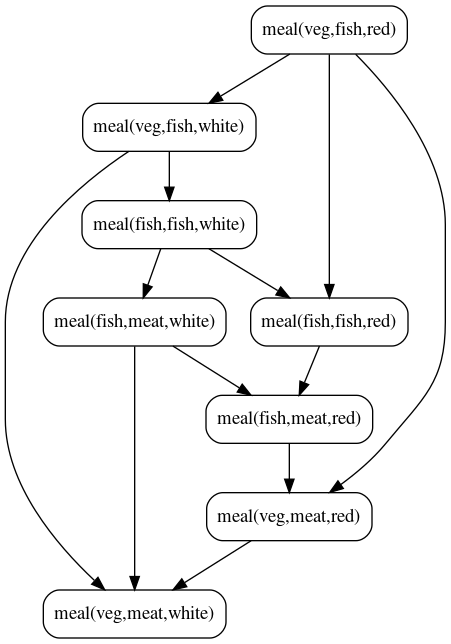
\includegraphics[width=0.6\linewidth]{ch3/cp-graph.png}
  \caption{Preference Structure of the Agent over \asc{meal/3}}
  \label{fig:cp-graph}
  
\end{figure}

\subsection{Goal Refinement via Preferences}
\label{ssec:goalref}
The integration of preferences into the BDI reasoning cycle can be implemented as a \textit{unifier ordering} step prior the \textit{plan selection}, that only applies when the triggering event contains unbounded variables. To achieve this, when the agent selects a partially unbounded event $\epsilon$, first it needs to find all the relevant unifiers by consulting the plan library, and then find all the applicable unifiers by consulting the belief base. Afterwards, the agent can create a partial ordering between the applicable unifiers. 

To extend the definition of section \ref{ssec:prefs} to unifiers, assuming $\epsilon$ is a partially unbound event and $(\sigma\delta),(\sigma\delta)'$ are two applicable unifiers for $\epsilon$, we say $(\sigma\delta) \succ (\sigma\delta)'$ satisfies a preference statement $G \succ G' \leftarrow C$ if $\epsilon(\sigma\delta)$ can be unified with $G$ and $\epsilon(\sigma\delta)'$ can be unified with $G'$. Given  $\Lambda$, a set of acyclic preference statements in this form, then we say $\Lambda \models (\sigma\delta) \succ (\sigma\delta)'$ iff $(\sigma\delta) \succ (\sigma\delta)'$ satisfies every active preference statement in $\Lambda$. We can then say $(\sigma\delta)$ is \textit{preferred} to $(\sigma\delta)'$ iff $\Lambda \not\models (\sigma\delta)' \succ (\sigma\delta)$. An then we can define the \textit{undominated} or \textit{most preferred} unifier:

\begin{definition}[Most preferred unifier]
\label{def:mpu}
A unifier $(\sigma\delta)$ is referred to as an \textit{undominated} or \textit{most preferred} unifier for an event $\epsilon$ iff $\sigma\delta$ is an applicable unifier for $\epsilon$ and for every other applicable unifier $(\sigma\delta)'$ we have $\Lambda \not\models (\sigma\delta)' \succ (\sigma\delta)$.
\end{definition}

Surprisingly, with this definition, finding the most preferred unifier is simple in a Prolog program as it matches well with how Prolog engines work. Normally in a Prolog program it is not easy to query if a fact holds with respect to every rule concerning that fact, but if a query about a fact fails, this means that all the rules about that fact have failed i.e, that the fact can not be proven. Thus, to find if a unifer $(\sigma\delta)$ is the most preferred one for an event $\epsilon$, it is enough to ask if for every other unifier $(\sigma\delta)'$, the query $(\sigma\delta)' \succ (\sigma\delta)$ fails. Intuitively, running this query for every unifier of $\epsilon$ will result in finding the most preferred unifier. More details on the implementation of this algorithm is presented in section \ref{sec:implementation}.

%Assuming $\Lambda$ is a set of acyclic (with respect to parent-child relations) preference relations over variables of $V$, and considering $o,o'$ are outcomes of $V$, then we say $\Lambda \models o \succ o'$ iff $o \succ o'$ satisfies every preference statement in $\Lambda$. 
%$\Lambda$ is satisfiable iff there exists a preference ranking $\succ$ over the outcomes of $V$ that each $o \succ o'$ satisfies each of the preference statements of $\Lambda$. It is said that $\Lambda \models o \succ o'$ iff $o \succ o'$ holds in every preference ordering that satisfies $\Lambda$. 
%Then $o$ and $o'$ can have one of the possible relations according to $\Lambda$: either $\Lambda \models o \succ o'$; or $\Lambda \models o' \succ o$; or $\Lambda \not\models o \succ o'$ and $\Lambda \not\models o \succ o'$. The third case means there is not enough information to prove either outcome is preferred.

%, then $\Lambda$ is satisfiable iff there exists a preference ranking $\succ$ over the applicable unifiers of $\epsilon$ that each $(\sigma\delta) \succ (\sigma\delta)'$ satisfies each of the preference statements of $\Lambda$. 
%it is said that $\Lambda \models (\sigma\delta) \succ (\sigma\delta)'$ iff $(\sigma\delta) \succ (\sigma\delta)'$ holds in every preference ordering that satisfies $\Lambda$.




%In this ordering, a an applicable unifier $(\sigma\delta)$ precedes another applicable unifier $(\sigma\delta')$ for $\epsilon$, if $\epsilon(\sigma\delta)$ is not dominated by $\epsilon(\sigma\delta)'$ according to the preferences. Note that this will result in a partial ordering and some unifiers may be incomparable depending on the preferences. 


%With this approach, %the normal plan selection can continue w.r.t. the re-ordered list of unifiers, but now, 
%the plan selection function can take into account the ordering between unifiers. Through the rest of the chapter, f
For simplicity, it is assumed that the agent uses the plan selection function typical in BDI frameworks, i.e. selecting the first applicable unifier for each event. This assumption means that the agent always uses an \textit{undominated} or \textit{most preferred} unifier to ground the variables of a (partially) abstract goal if this unifier exists, or reverts to the default behavior of selecting the first applicable unifier in case of inconsistencies with preferences that may result in situations that no unifier is the most preferred.
%Note that the event does not need to be fully grounded and it may be that the unifier $\sigma$ keeps some of the variables unbounded or even introduce new variables. As this unifier 



\subsubsection*{Example 4}
Consider again the agent script given in example 1, with the beliefs of example 2, and with the preferences of example 3. Assume that this agent receives an abstract event \asc{!go_order(L,M)}. Then, as in example 2, two applicable unifiers will be created. P1 will be applicable with the unifier \asc{{Loc/italian, Meal/M}} and P2 with the unifier \asc{{Loc/french, Meal/M}}. Because the agent has the belief \asc{at(french)}, we can see that the relation:
\begin{minted}[fontsize=\small]{prolog}
!go_order(italian,M) >> !go_order(french,M)
\end{minted}
can not be proven from the preferences (R8 and R9 can not conclude it) but the relation:
\begin{minted}[fontsize=\small]{prolog}
!go_order(french,M) >> !go_order(italian,M)
\end{minted}
can be proven to be true (based on R8), so
% \begin{minted}[fontsize=\small]{prolog}
% !go_order(french,M) >> !go_order(italian,M)
% \end{minted}
the \asc{{Loc/french, Meal/M}} is the single most preferred unifier and P2 will be selected as this is the only plan applicable with this unifier. Next, when the sub-goal \asc{!order(Meal)} is being considered, there are 8 applicable unifiers for plan P3, assuming the \asc{at(french)} belief still stands, and based on the given preference rules, the ordering in Fig.~\ref{fig:cp-graph} will apply, and then the most preferred unifier will be \asc{{S/veg, M/fish, W/red}}. This means that the abstract goal will be refined to \asc{!order(meal(veg,fish,red))} and consequently plan selection will instantiate the plan associated to it (P3).

\subsubsection*{Example 5}
To show how partially abstract goals would be grounded with this method, consider the same agent as before with the same set of preferences and beliefs, except this time the agent has the belief \asc{at(home)} instead of \asc{at(french)}, and the agent receives an event with ordering a meal with meat as the main course:
\begin{minted}[fontsize=\small]{prolog}
!go_order(L,meal(S,meat,W)). 
\end{minted}
This time plan P2 will be applicable with two unifiers:
\begin{minted}[fontsize=\small]{prolog}
{Loc/italian, Meal/meal(S,meat,W)}
{Loc/french, Meal/meal(S,meat,W)}
\end{minted}
because the agent has the belief \asc{at(home)}, the statement R8 is not active for any of the unifiers and based on the the statement R9, the Italian restaurant is preferred to any other restaurant as long as there is meat main course, so again while the relation:
\begin{minted}[fontsize=\footnotesize]{prolog}
!go_order(italian,meal(S,meat,W)) >> !go_order(french,meal(S,meat,W))
\end{minted}
can be proven (based on R9), but the relation:
\begin{minted}[fontsize=\footnotesize]{prolog}
!go_order(french,meal(S,meat,W)) >> !go_order(italian,meal(S,meat,W))
\end{minted}
can not be proven from the preference statements (R8 and R9 can not conclude it), so the first unifier will be the most preferred one and then P2 is selected with it. Next, assuming the \asc{move_to} action works correctly, the belief \asc{at(home)} will be retracted, \asc{at(italian)} will be added to the belief-base, and the sub-goal \asc{!order(meal(S,meat,W))} will be adopted. At this point (see the example in \cite{Boutilier2004}), based on the preference statements and agent's beliefs, the most preferred unifier will be \asc{{S/fish, M/meat, W/white}}, meaning the goal will be refined to \asc{!order(meal(fish,meat,white))}, and then the plan for this goal (P3) will be instantiated by the plan selection.

An interesting point in this example is the interaction between preference statements R1 and R9. In normal CP-Nets, these two statements makes the network cyclic: the preference over main dish is dependent on the location (R1), and the preference over the location depends on the main dish (R9). But in this work such preferences can be defined for two reasons: (1) \textit{framing}, meaning the two preferences, although being about the same variables, are defined in two different frames of choice, and (2) \textit{context}, meaning that as the agent resides and acts in a dynamic environment, it perceives changes and modifies its beliefs, which in turn modifies the agent's preferences, e.g. while the agent has the belief \asc{at(home)}, R1 and R2 are not active and so they are not part of unifier selection process. 

%\Mos{NEED TO WRITE ABOUT THE TEMPORAL ASPECT OF THIS EXAMPLE HERE OR LATER ON, IN NORMAL CP-NETS THIS IS A CYCLE, FOOD DEPENDED ON LOCATION AND LOCATION DEPENDED ON FOOD, BUT HERE BECAUSE THERE ARE DIFFERENT CHOICE POINTS ITS NOT A PROBLEM}

%\Gio{[Very interesting. I would write it here]} 

\section{Implementation\label{sec:implementation}}

This section presents a practical implementation
of the transformation method from CP-Theory logic to Prolog logic proposed in section \ref{sssec:transform}. 

\subsubsection*{Preference operator}
First, we need to express a preference statement $G1 \succ G2 \leftarrow C$, where $G1,G2$ are partially grounded terms with the same functor and arity. The mapping from CP-Theory statements to this statement is presented in section \ref{sssec:transform}. This binary operator $\succ$ will be introduced both into the syntax of the agent programming language and as a binary predicate into the belief base of the agent. In the syntax, the operator $\succ$ will be denoted as \asc{>>} making a relation such as $G1 \succ G2$ to be written as \asc{G1 >> G2}.
%Interestingly, as this operator is simply there to define a relation between two terms, it does not need any extra logic attached to it. In fact, this method can be implemented even without introducing a new operator to the syntax by instead using a predefined binary predicate such as \asc{preferred/2}, this way a preference relation $G1 \succ G2$ can be written as \asc{preferred(G1,G2)} instead. 
To write full contextually conditioned statements as $G1 \succ G2 \leftarrow C$, we can utilize the Prolog inference rules. The former preference statement can then be written as \asc{G1 >> G2 :- C}. %With this way of writing, at any point in run-time, given two partially ground terms \asc{g1,g2} then \asc{g1 >> g2} is considered a logical consequence of the belief base if there is a correct 

\subsubsection*{Applicability} Next, as the method is implemented by utilizing the belief-base of the agent, a modification is needed to allow preference statements about different types of \textit{goals} to be part of the belief base, as e.g. in the R8 statement from listing \ref{lst:prefs_1}. To do this, a supplementary predicate $applicable/2$ is introduced. When a preference statement $G1 \succ G2 \leftarrow C$ is defined where $G1$ and $G2$ are triggering events e.g. achievement goal ($!G$), test goal ($?G$), the preference statement is transformed at compile/interpretation time to:
\begin{equation*}
applicable(t,G1) \succ applicable(t,G2) \leftarrow C
\end{equation*}
where $t$ is a predefined atom describing the type of the event, e.g: the preference statement R8 in listing \ref{lst:prefs_1} will be rewitten as:
\begin{minted}[fontsize=\small]{prolog}
applicable(achievement,go_order(L,_)) 
    >> applicable(achievement,go_order(_,_)) 
    :- at(L).
\end{minted}
As this is a normal Prolog rule, it can be simply added to the belief base of the agent. Then, preference relations can be queried from any context, as e.g. the (meta-)preference R7 in listing \ref{lst:prefs_1}, in which a preference relation is used as the condition of another preference, or, more importantly, to exploit Prolog queries to find the most preferred unifier for abstract events.

\subsubsection*{Optimality}
Next, the algorithm should be implemented for finding an optimal outcome, that is, the most preferred unifier(s) for a partially abstract term. The algorithms originally introduced for CP-Nets and CP-Theories generate an optimal outcome by \textit{sweeping} through the network from top to bottom (i.e., from ancestors to descendants) setting each variable to its most preferred value given the instantiation of its parents. While these algorithms are efficient and intuitive, they are not applicable for the transformed Prolog-like rules. Unlike CP-Nets and CP-Theories, the preferential structure of an agent is not static because of the presence of extra-contextual conditions; also, with the new form of statements, the parent-child relation of the variables is not explicit anymore. For these reasons, new algorithms are needed that do not rely on the hierarchy of the variables but instead utilize the backtracking feature of Prolog. 

Looking at the definition \ref{def:mpu}, given a set of preference statements as Prolog rules in a belief base $B$, to prove that a unifier $(\sigma\delta)$ is the most preferred unifier for a partially unbound term (or event) $\epsilon$, it is sufficient to prove that for every other unifier $(\sigma\delta)'$ of that term, the relation $\epsilon(\sigma\delta)' \succ \epsilon(\sigma\delta)$ is not a logical consequence of $B$. Intuitively with the semantics of Prolog, this means that this relation could not be concluded from any of the preference statements of $B$. With this, a simple algorithm that can find the most preferred (or undominated) unifier(s) for a partially unbound term is a backtracking search that goes through every possible (partial) grounding of that term to find one where there is no other (partial) grounding of that term which is more preferred to it. Such algorithm can be implemented by adding the Prolog rule presented in Listing~\ref{lst:pref_alg} to the agent's belief base. The \asc{copy_term/2} is a standard predicate in many Prolog implementations that unifies \asc{G2} with a copy of \asc{G} in which all variables are replaced by new variables. 
\begin{listing}[!ht]
\begin{minted}[fontsize=\small]{prolog}
most_preferred(G) :- 
    copy_term(G, G2), G, 
    forall((G2, (G2 >> G) -> fail; true)).
\end{minted}
\caption{CP-Net reasoning algorithm implemented in Prolog}
\label{lst:pref_alg}
\end{listing}

% have been replaced by brand new variables, and all mutables by brand new mutables''. 
When this rule is queried with a partially unbound term \asc{G}, first a copy of \asc{G} is created as \asc{G2}, then the term \asc{G} itself is called, starting a backtracking search over all possible groundings of \asc{G}, and then \asc{forall/2} predicate starts a nested loop over all groundings of \asc{G2} and fails if it can find a grounding of \asc{G2} that \asc{(G2 >> G)}, otherwise if no such \asc{G2} is found it returns true meaning the current grounding of \asc{G} is the most preferred one. Also with how prolog queries work, if there is more than one most preferred (undominated) grounding, asking for more answers will return them.

There is one final rule needed to make this algorithm work which should be added to the belief base of the agent: \asc{T >> T :- !,fail.} which defines that a term can not be preferred to itself. With these rules added to the belief base, given a partially unbound term, we can run queries to find the most preferred unifier for that term. If we consider the example agent, querying the belief base with the term \asc{most_preferred(meal(S,M,W))} will give the result in one answer with the unifier \asc{{S/veg, M/fish, W/red}}. 

\subsubsection*{Embedding in the decision-making cycle}
Now that the belief base can answer queries about the most preferred unifier for a term, the next step is to allow the agent's reasoning engine to ask queries about the most preferred unifier for an event. To do this, the $applicable/2$ predicate that was defined before is used again. At compile/interpretation time, for each plan of the form $e : C \Rightarrow H$ a Prolog rule is added to the belief base of the agent in the form of:
\begin{equation*}
applicable(t,G) \leftarrow C
\end{equation*}
where $t$ is an atom that represents the type of the event $e$ and $G$ is the term associated with $e$. As an example, the rule for plan P1 is:
\begin{minted}[fontsize=\small]{prolog}
applicable(achievement,go_eat(L,M)) :-
    restaurant(L) & not at(L)
\end{minted}
Intuitively, at any moment in run-time, by querying this predicate, we can retrieve all possible applicable groundings of an event that can be concluded from the plan library and the belief base. For instance, by querying the term  \asc{applicable(achievement,go_eat(L,M))}
on the belief base of an agent with the beliefs, plans and preferences described in section \ref{sec:method}, the agent obtains two answers: \asc{{L/italian, M/M}} and \asc{{L/french, M/M}}. Then, by using this predicate with combination of \asc{most_preferred/2}, the agent can find the \textit{most preferred applicable unifier} for an event. This is possible because the preference statements about events were already transformed with the \asc{applicable} predicate. Considering our running example, by querying the term 
\begin{minted}[fontsize=\small]{prolog}
most_preferred(applicable(achievement,go_eat(L,M)))
\end{minted}
only one answer \asc{{L/french, M/M}} will be returned. Now to embed the goal refinement step into the agent reasoning cycle.
%is trivial, yet depending on the framework at hand. In general, only minimal modifications are required: 
After the event selection step, if the selected event $\epsilon$ contains free variables, then the most preferred unifier(s) should be found for this event by querying the belief base of the agent with the aforementioned method, and the resulting answer(s) are sent to the plan selection function.


\subsubsection*{Complexity}
%Calculating the time complexity of the algorithm is rather simple, 
The core of the method is the rule for the predicate \asc{most_preferred/1}, and this rule has two nested backtracking loops over the possible groundings of the input term. In the worst case scenario, each two groundings of a term should be queried with all of the preference statements associated to that rule. Then, for a term $T$, if the there are $n$ number of possible groundings at any time, and there are $m$ preference statements over $T$, then, in the worst case scenario, the time complexity of finding the most preferred unifier will be $n^2 \times m$. 

%\Gio{[What about the complexity of CP-nets/CP-theories? I would also add something like. Such worst-case scenario can be reduced by optimizing the relative positions of preferential rules and groundings in the belief base, for instance by exploiting statistical information concerning their applicability or relevance for the decision-making cycle. Note that this information depends on the coupling agent-environment, and a structural change in the workings of one of the two would demand a recomputation of the relative positions of rules and facts.]}



\section{Discussion and conclusion}
\label{sec:discuss}
This chapter contributes to recent efforts to integrate preferences into BDI agents. Despite the `D' in the acronym, desires play a limited role in contemporary BDI agent platforms, as they are generally conflated to goals (procedural or declarative). This chapter showed that by interacting adequately with the belief base and plan library of the agent, abstract goals can be refined taking into considerations the agent's preferences. Stated differently, preferences act here as background desires modifying/impacting goals, playing the role in turn of contingent desires. (Note that in general the literature suggests that preferences are
derived from desires \cite{Lorini2017}; for our purposes, however, we discovered that the two can be seen as filling the same functional niche.) 

Although this work illustrated the use of preferences focusing on a single agent and on goal refinement, preference statements can be relevant in other contexts too. For instance, MAS frameworks allow agents to communicate and transmit their beliefs to each other. Leveraging the present proposal, because preference statements are implemented as beliefs, agents can directly communicate their preferences to other agents. This can be very useful e.g. in social simulation or social learning contexts, where the agents may need to decide to act (or not to act) depending on both their own and other agents' preferences. Another interesting use-case for this approach could be the implementation of normative agents, utilizing preference both to capture personal and societal norms (see the use of CP-nets for deontic logic in \cite{Sartor2020}).

Preference statements introduced in this work are in a form processable in Prolog logic programs. We have shown that a subset of this form can be used to express pure CP-Theory preferences. However, this new form can also be used to express contextually conditioned and parameterized preferences, resulting in much more flexibility than pure CP-Theories. Consider for instance the statement R8 in example 3: ``\textit{I prefer the place I am already at}''; that depends completely on the state of the agent in the environment and, if the environment is unknown and unpredictable, so will be the preference statement. 
Also, unlike CP-Theories that are fully qualitative, with the proposed form quantitative preferences can be expressed by using arbitrary arithmetic equations in the context condition of preferences; e.g: consider a statement ``\textit{I prefer a cheaper restaurant to a more expensive one}'' that can easily be expressed in this form with an arithmetic comparison as the condition of the statement.
But this flexibility %comes also
%Although this flexibility is needed to express the complex preferences of agents that acts in highly dynamic and unpredictable environments, it 
comes at the cost of static verifiability. Many of the preferences that can be expressed in the proposed representational model %could 
cannot be statically verified or predicted easily prior to run-time. The redeeming aspect of this problem is that static verification of dynamic agents is well-known to be a challenging task, especially in dynamic environments \cite{Fisher2020,Ferrando2019}. This explains the existence of run-time verification approaches for agent programming frameworks, and probably the most notable works that adopt a (semi-)formal run-time model checking approach to verification are those of the AJPF/MCAPL framework \cite{Dennis2012,Dennis2016}. These approaches are in principle also usable for agents that are enhanced with preferences.

Finally, one of the main requirement behind this work is accessible usability. The transformation method from CP-Theory preference statements to Prolog-like programs has been conceived to enable its use almost directly with AgentSpeak(L)-like frameworks \cite{Bordini2005,ASTRA,mohajeriparizi_2020_run,Aschermann2018}. Indeed, no extra reasoning component is introduced, all the preference reasoning and algorithms required for goal refinement is done through beliefs and inferential rules. Furthermore, unlike many of the works that embed preferences into BDI frameworks, e.g. \cite{Visser2011,Visser2016,Dasgupta2010,Mohajeri2019,Mohajeri2020}, this approach does not require any extra annotation of the agent's script with information about effects of plans or actions and thus makes it more accessible for the designer. 

A concrete Prolog implementation of ordering queries of CP-Nets/CP-Theories was presented, and a working proof of concept for this approach is publicly available\footnote{anonymized}. Analyzing its complexity, we showed that the proposed algorithm run in polynomial time. Such worst-case scenario could be however reduced by optimizing the relative positions of preferential rules and groundings in the belief base, for instance by exploiting statistical information concerning their applicability or relevance for the decision-making cycle. %Note that this information depends on the coupling agent-environment, and a structural change in the workings of one of the two would demand a recomputation of the relative positions of rules and facts.

% We believe that for these reasons, this method can be easily implemented in many of the existing BDI frameworks and a working proof of concept for this approach have been implemented\footnote{anonymized}.


